\loesung{
%
%\begin{table}[ht]
%	\centering
%	\begin{tabular}{lcc|c}
%		\hline
%		 & Hepatitis A & no Hepatitis A & $\Sigma$\\
%		\hline
%		Salsa eaten & $218 (a)$ & $45 (b)$ & $263$ \\
%		Salsa not eaten & $21 (c)$ & $85 (d)$ & $106$\\
%		\hline
%		$\Sigma$ & $239$ & $130$ & $369$\\
%		\hline
%	\end{tabular}
%\end{table}

\begin{table}[ht]
	\centering
	\begin{tabular}{rrrrrr}
		\hline
		& WINTER & SPRING & SUMMER & FALL & $\Sigma$ \\ 
		\hline
		$y$=0 & 174.00 & 111.00 & 98.00 & 128.00 & 511.00 \\ 
		$y$=1 & 7.00 & 73.00 & 90.00 & 50.00 & 220.00 \\ 
		$\Sigma$ & 181.00 & 184.00 & 188.00 & 178.00 & 731.00 \\ 
		\hline
	\end{tabular}
\end{table}

\begin{enumerate}[a)]
	\item Odds for ``high number of bike rentals'' vs. ``low to medium number of bike rentals'' in winter: $$\text{odds} = \frac{P(y=1\, | \,\texttt{season}=\text{WINTER})}{P(y=0\, | \,\texttt{season}=\text{WINTER})} = \frac{7}{174} = 0.04 $$
	\textbf{Interpretation:} In winter the occurrence of \texttt{cnt} $> 5531$ ($y=1$) is $0.04$ times as likely as \texttt{cnt} $\leq 5531$ ($y=0$), the odds are $1:25$, which means ``$y=0$'' is 25 times as likely than ``$y=1$''.
    
	\item\label{ex_sol:logreg_GLM_single_feature_oddsratio_interpret}
    Odds Ratio of spring vs. winter: 
	\begin{align*}
		\text{odds ratio} 
		&= \frac{P(y=1\, | \,\texttt{season}=\text{SPRING})\,/\,P(y=0\, | \,\texttt{season}=\text{SPRING})}{P(y=1\, | \,\texttt{season}=\text{WINTER})\,/\,P(y=0\, | \,\texttt{season}=\text{WINTER})} \\
		&= \frac{73/111}{7/174} = 16.35
	\end{align*}

    For summer we get
    \[
    \text{odds ratio} 
    = \frac{P(y=1\, | \,\texttt{season}=\text{SUMMER})\,/\,P(y=0\, | \,\texttt{season}=\text{SUMMER})}{P(y=1\, | \,\texttt{season}=\text{WINTER})\,/\,P(y=0\, | \,\texttt{season}=\text{WINTER})}
    = \frac{90/98}{7/174} = 22.83,
    \]

    and for fall:
    \[
    \text{odds ratio} 
    = \frac{P(y=1\, | \,\texttt{season}=\text{FALL})\,/\,P(y=0\, | \,\texttt{season}=\text{FALL})}{P(y=1\, | \,\texttt{season}=\text{WINTER})\,/\,P(y=0\, | \,\texttt{season}=\text{WINTER})}
    = \frac{50/128}{7/174} = 9.71.
    \]
    
	\textbf{Interpretation:} The chances (the odds) of having "high bike rentals" are $16.35$ times higher in season SPRING compared to the reference category (WINTER).
    As in winter the odds of ``$y=0$'' are $25:1$, this means in spring they are roughly $(25:16):1$, which means roughly $5:3$.
    Similarly, in summer the odds are $22.83$ times higher that in winter, which means that in summer they are close to $1:1$ (since in winter they were $1:25$), so the chances in summer are roughly 50-50.

	\item\label{ex_sol:logreg_GLM_single_feature}
    Table:
	\begin{table}[!ht]
		\centering
		\begin{tabular}{rrrr}
			\hline
			& Estimate & Std. Error & Pr($>$$|$z$|$) \\ 
			\hline
			(Intercept) & -3.2131 & 0.3854 & 0.0000 \\ 
			seasonSPRING & 2.7941 & 0.4138 & 0.0000 \\ 
			seasonSUMMER & 3.1280 & 0.4121 & 0.0000 \\ 
			seasonFALL & 2.2731 & 0.4199 & 0.0000 \\ 
			\hline
		\end{tabular}
	\end{table}

	The intercept gives the odds for ``high number of bike rentals'' vs. ``low to medium number of bike rentals'' for the default category, in winter: exp$(-3.2131) = 0.04$. Interpretation as in a).
	
	Regarding the estimate of seasonSPRING (and analogous for all the other seasons): $\text{odds ratio (when season changes from winter to spring)} = \text{exp}(2.7941) =  16.35$. Interpretation as in b).

    \item\label{ex_sol:logreg_GLM_more_features}

    \begin{enumerate}[(i)]
    
        \item\textbf{Offset.}
        $
        \delta=
        (-0.0627)(62.79)
        +(-0.0925)(12.76)
        +(0.0166)(365.00)
        =\boxed{0.94}.
        $
        
        \item\textbf{Probabilities.}        
        \[
        \text{Effective intercept: } \beta_0+\delta=-7.58
        \qquad
        \eta(x_1)=-7.58 + 0.29\,x_1,
        \qquad
        p(x_1)=\sigma\!\bigl(\eta(x_1)\bigr).
        \]
        
        \begin{center}
        \begin{tabular}{cccc}
        \toprule
        \(x_1\) (\si{\celsius}) & \(\eta(x_1)\) & \(p(x_1)\) \\
        \midrule
        10 &  -4.677 & 0.009 \\
        15 &  -3.227 & 0.038 \\
        20 &  -1.777 & 0.144 \\
        25 &  -0.327 & 0.419 \\
        30 &   1.123 & 0.755 \\
        35 &   2.573 & 0.929 \\
        \bottomrule
        \end{tabular}
        \end{center}
        
        \item\textbf{Derivation of the marginal effect.}
        
        \textbf{Goal:} Compute the instantaneous change in the predicted probability  
        when temperature \(x_{1}\) increases, holding all other features constant:
        \[
        \frac{\partial p}{\partial x_{1}}
           \;=\;
           \frac{\partial}{\partial x_{1}}
           \sigma\!\bigl(\eta\bigr),
           \qquad
           \eta=\beta_{0}+\delta+\beta_{1}x_{1},
        \]
        where \(p=\sigma(\eta)=\bigl(1+e^{-\eta}\bigr)^{-1}\) and  
        \(\delta\) collects the fixed contributions of the remaining covariates.
        
        \begin{enumerate}
            \item \textbf{Applying the chain rule}
            \[
            \frac{\partial p}{\partial x_{1}}
             \;=\;
             \frac{\partial \sigma(\eta)}{\partial \eta}\,
             \frac{\partial \eta}{\partial x_{1}} .
            \]
            
            \item \textbf{Derivative of the sigmoid}
            
            We begin with the definition of the sigmoid function:
            \[
            \sigma(\eta) = \frac{1}{1 + e^{-\eta}}.
            \]
            
            We aim to compute its derivative with respect to \( \eta \):
            \[
            \frac{d}{d\eta} \left( \frac{1}{1 + e^{-\eta}} \right).
            \]
            
            Rewriting using the power rule:
            \[
            \sigma(\eta) = (1 + e^{-\eta})^{-1},
            \]
            so by the chain rule:
            \[
            \frac{d\sigma}{d\eta}
              = -1 \cdot (1 + e^{-\eta})^{-2} \cdot \frac{d}{d\eta}(1 + e^{-\eta})
              = \frac{e^{-\eta}}{(1 + e^{-\eta})^2}.
            \]
            
            To express this in terms of \( \sigma(\eta) \), note:
            \[
            \sigma(\eta) = \frac{1}{1 + e^{-\eta}},
            \quad\text{and}\quad
            1 - \sigma(\eta) = \frac{e^{-\eta}}{1 + e^{-\eta}}.
            \]
            
            Hence:
            \[
            \sigma(\eta)\,(1 - \sigma(\eta)) = \frac{1}{1 + e^{-\eta}} \cdot \frac{e^{-\eta}}{1 + e^{-\eta}} = \frac{e^{-\eta}}{(1 + e^{-\eta})^2}.
            \]
            
            So the derivative simplifies to:
            \[
            \frac{\partial p}{\partial \eta}
              = \frac{d\sigma}{d\eta}
              = \sigma(\eta)\,(1 - \sigma(\eta))
              = p\,(1 - p).
            \]
            
            \item \textbf{Derivative of the linear predictor}
            \[
            \frac{\partial \eta}{\partial x_{1}}
              =\beta_{1},
            \qquad
            \text{because } \eta=\beta_{0}+\delta+\beta_{1}x_{1}.
            \]
            
            \item \textbf{Combining the two results}
            \[
            \boxed{\displaystyle
              \frac{\partial p}{\partial x_{1}}
                = p\,(1-p)\,\beta_{1}} .
            \]
            
            \item \textbf{Interpretation}
            
            The factor \(p(1-p)\) is maximal at \(p=0.5\) and vanishes as \(p\to0\) or \(p\to1\), illustrating that \(x_{1}\) has the largest marginal effect when the model is most uncertain and a negligible effect in the extreme–probability regions, when the model is extremely confident.
            The coefficient
            \(\beta_{1}\) scales this intrinsic sensitivity, so the overall effect is
            \emph{context‐dependent}: It varies with the current value of the linear predictor
            through \(p\).
        \end{enumerate}
        
        The scaling term \(p(1-p)\le 0.25\) peaks at \(p=0.5\), explaining
        why the same coefficient \(\beta_{1}=0.29\) produces the largest
        probability change near the mid-range and almost none in the tails.
        
        % \[
        % \frac{dp}{dx_1}
        % =\frac{dp}{d\eta}\,\frac{d\eta}{dx_1}
        % \;\;=\;
        % \sigma(\eta)\bigl(1-\sigma(\eta)\bigr)\,\beta_1
        % \;=\; p(1-p)\beta_1 .
        % \]
        
        % Steps:
        
        % 1. \(p=\sigma(\eta)\), \(\dfrac{d\sigma}{d\eta}=\sigma(1-\sigma)\).
        % 2. \(\eta=\beta_0+\delta+\beta_1x_1 \;\Longrightarrow\; d\eta/dx_1=\beta_1\).
        
        \item\textbf{Numeric marginal effects:}
        $
        dp/dx_1 = p(1-p)\beta_1 = 0.29\,p(1-p).
        $
        
        $\Rightarrow$ Largest effect occurs near \(x_1\approx30^\circ\text{C}\) where \(p\approx0.5\).
        
        \begin{center}
        \begin{tabular}{ccc}
        \toprule
        \(x_1\) & \(p\) & \(dp/dx_1\) \\
        \midrule
        15 °C & 0.038 & 0.011 \\
        30 °C & 0.755 & \textbf{0.054} \\
        35 °C & 0.929 & 0.019 \\
        \bottomrule
        \end{tabular}
        \end{center}
        
        %\textit{R verification}
        
        % \begin{verbatim}
        % beta0 <- -8.52; beta1 <- 0.29
        % delta <- -0.06266594*62.79 - 0.09247547*12.76 + 0.01659578*365
        % T <- c(10,15,20,25,30,35)
        % eta <- beta0 + delta + beta1*T
        % p   <- plogis(eta)
        % dp  <- p*(1-p)*beta1
        % data.frame(T, eta=round(eta,3), p=round(p,3), dp=round(dp,3))
        % \end{verbatim}

        \textbf{Visualization of the marginal effect:}
        \begin{center}
            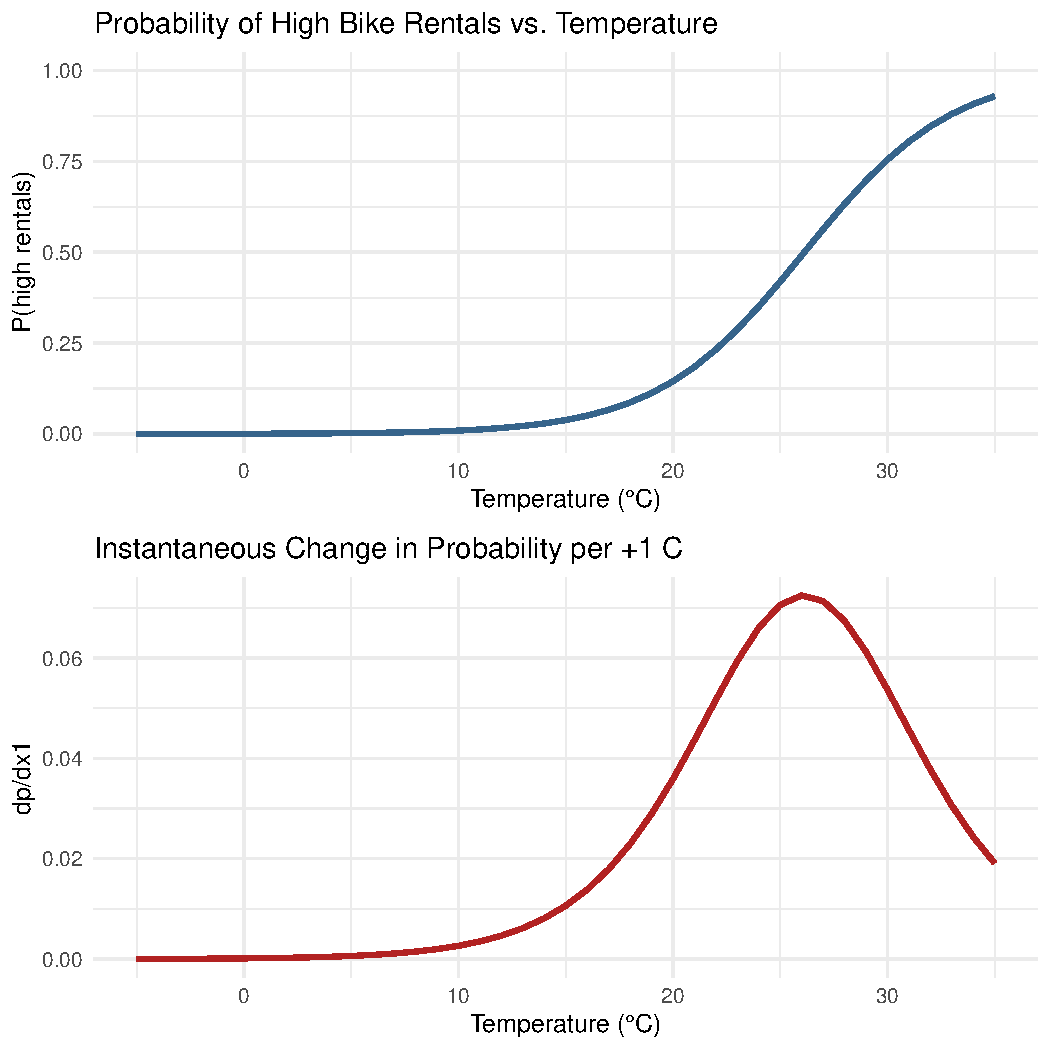
\includegraphics[width=.8\linewidth]{figure/logistic_reg_bike_plot_marginal_effect.pdf}
        \end{center}

        \textbf{Side note:} The curve for the probability is actually a PDP (see later in chapter on feature effects), because it shows the marginal effect of a single feature when all other features are averaged.
        If other fixed values are taken for the other features (e.g. values of some fixed single data point), the offset changes, in which case the sigmoid curve always looks the same and is only shifted depending on the other values.
        This is the difference between a PDP and an ICE plot, which we will discuss later in more detail.
        
        \item\textbf{Classification} at threshold 0.5:
        Predicted “high-rental” for temperatures with \(p\ge0.5\):
        \(\boxed{30^\circ\text{C},\,35^\circ\text{C}}\).

    \end{enumerate}

    \newpage
    
	\item Table:	
	\begin{table}[ht]
		\centering
		\begin{tabular}{rrrr}
			\hline
			& Estimate & Std. Error & Pr($>$$|$z$|$) \\ 
			\hline
			(Intercept) & -8.5176 & 1.2066 & 0.0000 \\ 
			seasonSPRING & 1.7427 & 0.5977 & 0.0035 \\ 
			seasonSUMMER & -0.8566 & 0.7660 & 0.2635 \\ 
			seasonFALL & -0.6417 & 0.5543 & 0.2470 \\ 
			temp & 0.2902 & 0.0391 & 0.0000 \\ 
			hum & -0.0627 & 0.0124 & 0.0000 \\ 
			windspeed & -0.0925 & 0.0305 & 0.0024 \\ 
			days\_since\_2011 & 0.0166 & 0.0014 & 0.0000 \\ 
			\hline
		\end{tabular}
	\end{table}

    Again, look at your interpretations of the \(\beta\)-coefficients and of the effects of single features from parts \ref{ex_sol:logreg_GLM_single_feature}) and \ref{ex_sol:logreg_GLM_more_features}).
    What changes now in the full model?
	
	If all features are considered in the model, the $\beta$-value for the intercept is almost the same as in the second model and much higher in absolute terms than in the first model.
    Compared to part \ref{ex_sol:logreg_GLM_single_feature}), the odds change to exp($-8.5176) = 0.0002$, i.e. the probability of ``high number of bike rentals'' is (on average!) even less in winter when considering the full model compared to the one only containing feature \texttt{season}. Also, the average higher chance / higher odds of having "high bike rentals" in season SPRING compared to WINTER declined to exp($1.7427)=5.71$ (vs. $16.35$ in part \ref{ex_sol:logreg_GLM_single_feature_oddsratio_interpret}) in the smaller model).

    Comparing to part \ref{ex_sol:logreg_GLM_more_features}), one can observe that the estimates for all the coefficient stay almost the same, and additionally including the feature \texttt{season} seems to have no effect on the overall model.
    We can also observe very high p-values for the estimates of the different \texttt{season} categories, and low p-values for all the other features and the intercept.
    Hence, when considering all features, the data does not really provide evidence for a significant effect of the season on the number of bike rentals, and one should evaluate whether the feature \texttt{season} should be included in the model at all.
    
    This is very different conclusion compared to part \ref{ex_sol:logreg_GLM_single_feature})
    maybe has to do with the fact that the season is correlated with the temperature and the other weather-related features, so replacing the feature \texttt{season} with these other features is almost already enough for the model, and the remaining effect of the season alone is very small.

    The interpretation of the other features can also be done in terms of the odds ratio, analogously to part \ref{ex_sol:logreg_GLM_single_feature}), or in terms of the marginal feature effect or feature effect change, as in part \ref{ex_sol:logreg_GLM_more_features}), although these interpretations actually don't change at all compared to \ref{ex_sol:logreg_GLM_more_features}), since the corresponding coefficient estimates also did not change at all.

\end{enumerate}
}
